\documentclass[11pt,letterpaper]{article}

% Page and text formatting
\usepackage[margin=1in]{geometry}
\usepackage[T1]{fontenc}
\usepackage{lmodern}
\usepackage{microtype}
\usepackage{setspace}
\setstretch{1.10}
\setlength{\parindent}{0pt}
\setlength{\parskip}{0.45em}

% Figures, tables, and SQL
\usepackage{graphicx}
\graphicspath{{./}{../receipts/}}
\usepackage{amsmath,amssymb}
\usepackage{array,tabularx}
\usepackage{enumitem}
\usepackage{listings}
\usepackage[table]{xcolor}
\usepackage{placeins}
\usepackage{caption}
\usepackage{float}
\usepackage[hidelinks]{hyperref}
\setlist[itemize]{leftmargin=*,itemsep=0.15em,topsep=0.25em}

\lstdefinestyle{projectSQL}{
    language=SQL,
    basicstyle=\ttfamily\scriptsize,
    keywordstyle=\color{blue!50!black}\bfseries,
    commentstyle=\color{gray!75!black}\itshape,
    stringstyle=\color{teal!60!black},
    breaklines=true,
    breakatwhitespace=false,
    columns=fullflexible,
    keepspaces=true,
    showstringspaces=false,
    frame=single,
    rulecolor=\color{black!30},
    framesep=5pt,
    aboveskip=0.5em,
    belowskip=0.5em
}
\lstset{style=projectSQL}

\title{Supermarket Chain Database Web Application\\COSC 3380 --- Project Report}
\author{Matthew Dulworth \and Javier Puentes Leiva}
\date{Fall 2026}

\begin{document}
\maketitle

\section{Introduction}

This project implements a database-backed web application for a chain of 100 supermarkets across multiple states. It simulates product sales, store-specific inventory, tax calculations, and cash or card payments. The application uses PostgreSQL for data storage, Node.js and Express for the backend, and HTML and JavaScript for the frontend.

The supermarket and bank are separate databases. The web interface supports customer checkout, back-office reports, database administration, random checkout simulation, and concurrent customers. Transactions, row locking, and two-phase commit help keep purchases, inventory, and bank balances consistent.

\section{Database Design and Final ER Model}

\subsection{Database Structure}

The supermarket database contains seven related tables; the bank database contains one. Their responsibilities are summarized below.

\begin{center}
\small
\begin{tabularx}{\textwidth}{@{}>{\bfseries}p{0.24\textwidth}X@{}}
\hline
Table & Purpose \\ \hline
Tax & State sales tax rates \\
Department & Product categories \\
Store & Store locations, contact details, and aisles \\
Item & Product SKU, department, and tax/weight flags \\
Inventory & Product price, stock, and aisle by store \\
Store Transaction & Purchase date, store, payment method, and total \\
Item Sale & Products, quantities, and unit prices within each purchase \\
Account (bank) & Account numbers, balances, and account type (customer, or the supermarket's own account) \\ \hline
\end{tabularx}
\end{center}

\subsection{ER Design Iterations}
\label{sec:er-iterations}

The ER model was developed top-down over three iterations; all diagrams were drawn in draw.io.

\textbf{Initial design (brainstorm).} The first draft (Figure~\ref{fig:er-initial}) listed every candidate entity found on the receipts and in the assignment: customer, department, item, inventory, aisle, receipt, store, payment, employee, transaction, tax, and items sold, plus a bank account in a separate database. Most entities had only a key and one or two attributes, and several overlapped (receipt, payment, and transaction all described the same purchase).

\textbf{Preliminary design.} The second version (Figure~\ref{fig:er-prelim}) merged receipt and payment into a single \texttt{Transaction} entity carrying the payment method, bank account, amount, and time. Customer was dropped because a cash register does not identify customers, and the separate aisle entity became an attribute. \texttt{Item\_sales} and \texttt{Inventory\_and\_price} appeared as the two associative entities with composite keys, and multiplicities were added to every relationship. \texttt{Employee} remained but was not connected to anything.

\textbf{Final design.} The final model (Figure~\ref{fig:final-er}) made the following changes:
\begin{itemize}
    \item \texttt{Employee} was removed because no checkout or report used it.
    \item \texttt{priced\_by\_weight} moved from \texttt{Department} to \texttt{Item}. Pricing by weight is a property of a product, not a department (the produce department sells both bagged and loose items), so keeping it on \texttt{Department} would have made a department-level fact wrongly determine an item-level one.
    \item The separate \texttt{weight} and \texttt{count} columns in \texttt{Item\_sales} were combined into one \texttt{quantity\_sold} (pounds or units, interpreted through \texttt{priced\_by\_weight}), removing a pair of mutually exclusive nullable columns.
    \item \texttt{aisle\_no} was added to \texttt{inventory}, since the same product can sit in different aisles at different stores, and \texttt{aisles} was added to \texttt{store}.
    \item Store \texttt{address} was split into \texttt{street}, \texttt{city}, and \texttt{zip\_code} so reports can group and filter by city.
    \item Tables and columns were renamed to consistent snake\_case (\texttt{store\_transaction}, \texttt{item\_sale}, \texttt{inventory}).
\end{itemize}

\begin{figure}[H]
    \centering
    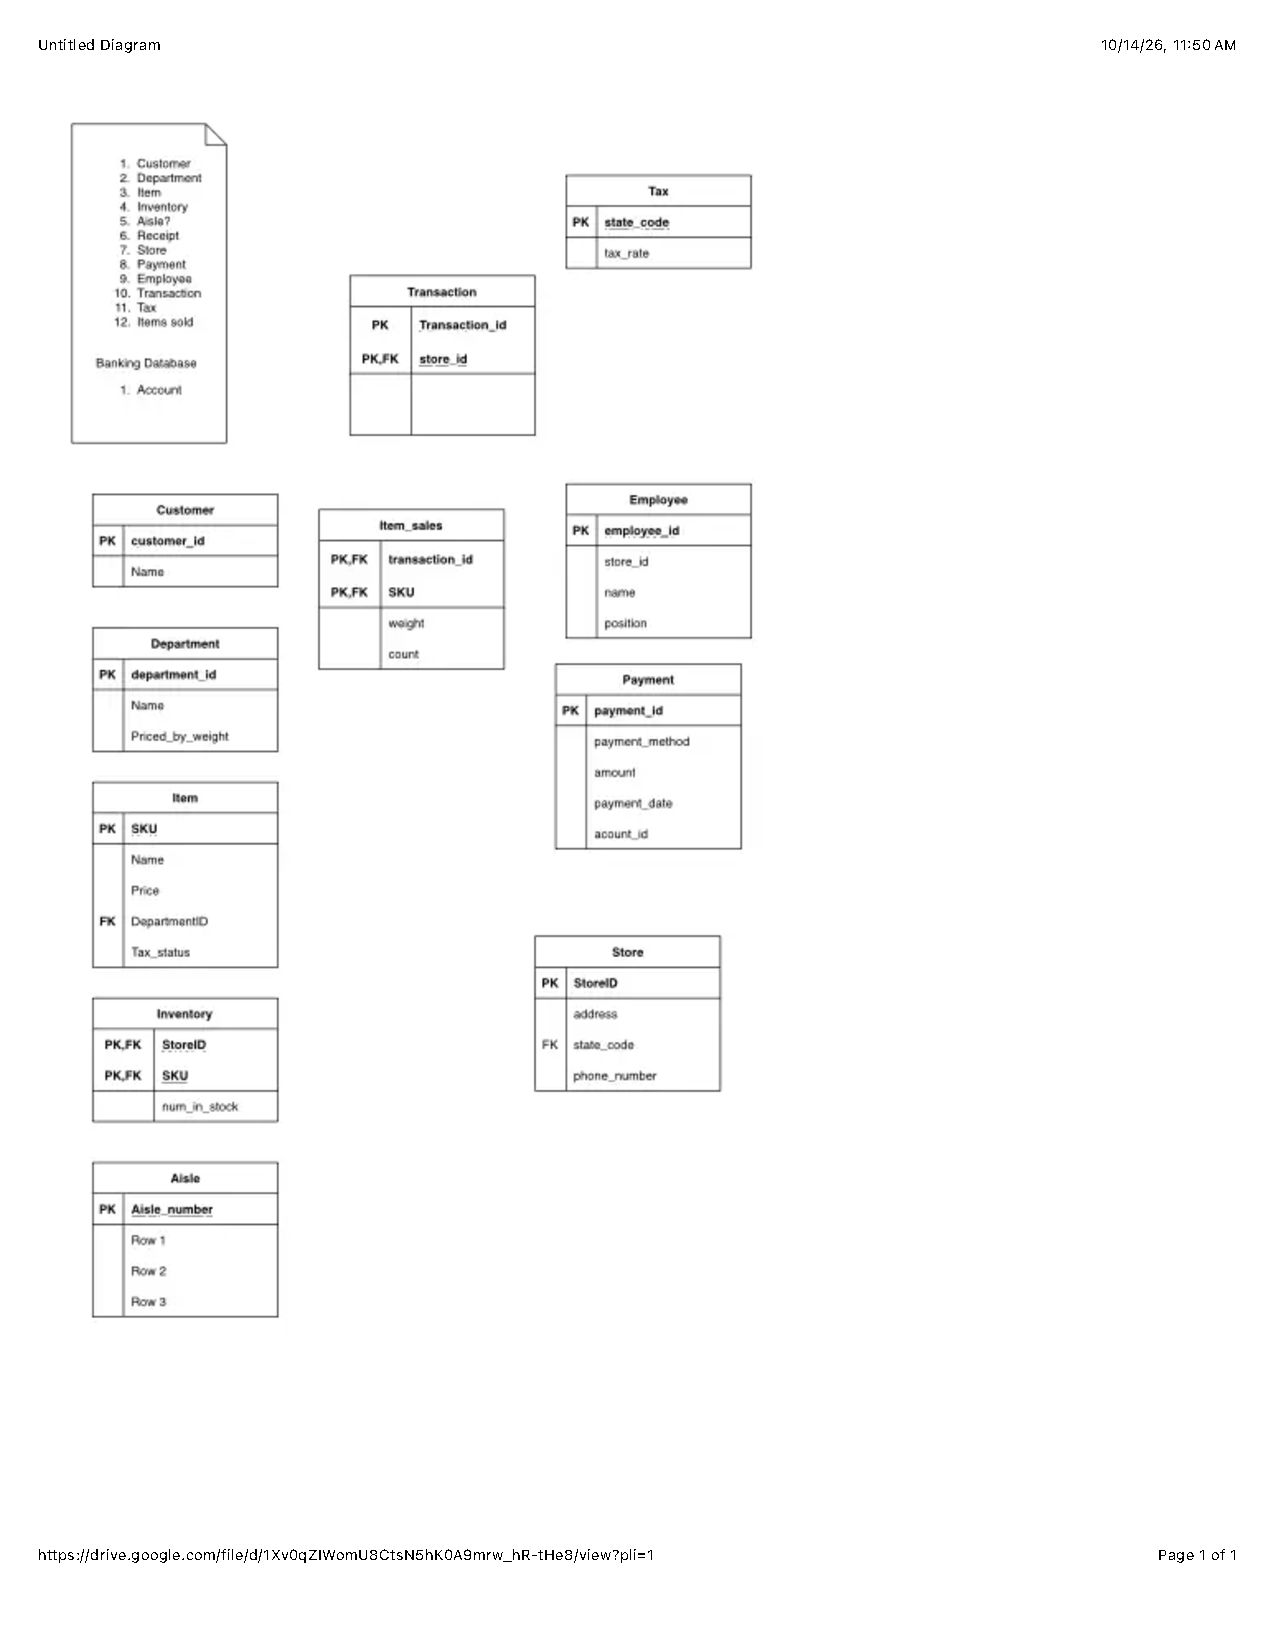
\includegraphics[width=0.55\textwidth,trim=0 60 0 30,clip]{initial thoughts.pdf}
    \caption{Initial ER Design (brainstorm)}
    \label{fig:er-initial}
\end{figure}

\begin{figure}[H]
    \centering
    \includegraphics[width=0.90\textwidth,height=0.42\textheight,keepaspectratio]{v2.png}
    \caption{Preliminary ER Design}
    \label{fig:er-prelim}
\end{figure}

\subsection{Final ER Model}

Figure~\ref{fig:final-er} shows the final supermarket ER model, which contains seven tables. The main one-to-many relationships are: one state tax record can apply to multiple stores; one store can have multiple transactions; and one department can contain multiple items. Each transaction belongs to one store, each item belongs to one department, and each store references one state tax record.

The \texttt{Inventory} table connects stores and items, allowing the same product to have different prices, stock quantities, and aisle locations at different stores. Its composite primary key, \texttt{(sku, store\_id)}, uniquely identifies each store--product combination. Similarly, \texttt{Item Sale} connects transactions and items, recording the quantity and unit price for each purchased product. Its composite primary key is \texttt{(transaction\_id, sku)}. These two tables implement the many-to-many relationships between stores and items, and between transactions and items.

Foreign keys enforce the relationships shown in the diagram, while \texttt{tax\_exempt} and \texttt{priced\_by\_weight} in \texttt{Item} determine how products are handled during checkout. A completed purchase consists of one transaction record and its corresponding item-sale records.

\begin{figure}[H]
    \centering
    \includegraphics[width=0.95\textwidth,height=0.49\textheight,keepaspectratio]{v3.png}
    \caption{Final Supermarket ER Model}
    \label{fig:final-er}
\end{figure}

The bank is modeled separately with the \texttt{Account} table (Figure~\ref{fig:bank-er}), whose primary key is \texttt{account\_number} and whose \texttt{balance} stores available funds. For card purchases, \texttt{store\_transaction.account\_id} identifies the bank account; for cash purchases, it is null. Because the databases are separate, this association is checked by the application rather than a cross-database foreign key.

The \texttt{account\_type} attribute distinguishes customer accounts from the supermarket chain's own account. Account 9000 is reserved for the supermarket, and a CHECK constraint ties that number to the \texttt{supermarket} type. Every completed sale, cash or card, credits this account, so the bank records the money the chain receives as well as the money customers pay.

\begin{figure}[H]
    \centering
    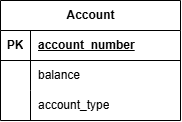
\includegraphics[width=0.32\textwidth]{bank.png}
    \caption{Bank Database ER Model}
    \label{fig:bank-er}
\end{figure}
\FloatBarrier

\section{Receipt Analysis}

Five receipts from H-E-B, Target, Tesco, Trader Joe's, and Whole Foods Market were examined to identify the fields needed for checkout and sales records. The original receipts appear in Appendix~\ref{app:receipts}.

\begin{center}
\small
\begin{tabularx}{\textwidth}{@{}>{\bfseries}p{0.19\textwidth}X@{}}
\hline
Receipt & Relevant observation \\ \hline
H-E-B & Weighted chestnuts, coupon savings, and card payment \\
Target & Multiple departments, discounts, and tax classifications \\
Tesco & Items sold by weight, VAT rates, and a different currency \\
Trader Joe's & Unit quantities, item prices, and payment totals \\
Whole Foods & Weighted produce, discounts, and tax details \\ \hline
\end{tabularx}
\end{center}

These examples informed the \texttt{Item}, \texttt{Inventory}, \texttt{Item Sale}, \texttt{Store Transaction}, and \texttt{Tax} tables. The table below shows where each field common to the receipts is stored.

\begin{center}
\footnotesize
\begin{tabularx}{\textwidth}{@{}>{\raggedright\arraybackslash}p{0.25\textwidth}>{\raggedright\arraybackslash}p{0.37\textwidth}>{\raggedright\arraybackslash}X@{}}
\hline
Receipt field & Stored in & Notes \\ \hline
Store name, address, phone & \texttt{store} & One row per location; \texttt{state\_code} links to the tax rate. \\
Date and time & \texttt{store\_transaction.\allowbreak date\_and\_time} & Defaults to the time of checkout. \\
Item description / product code & \texttt{item.name}, \texttt{item.sku} & SKU identifies the product chain-wide. \\
Department heading (Target) & \texttt{item.department\_id} $\rightarrow$ \texttt{department} & Used by the top-seller report. \\
Shelf price & \texttt{inventory.price} & Varies by store. \\
Price paid on the line & \texttt{item\_sale.unit\_price} & Copied from inventory at sale time. \\
Quantity or weight (e.g.\ ``1.42 lb @ \$/lb'') & \texttt{item\_sale.quantity\_sold} & Units or pounds, per \texttt{item.priced\_by\_weight}. \\
Taxable / non-taxable flag & \texttt{item.tax\_exempt} & Groceries vs.\ general merchandise. \\
Tax rate & \texttt{tax.tax\_rate} & One rate per state. \\
Total & \texttt{store\_transaction.\allowbreak total\_amount} & Stored snapshot (see Section~\ref{sec:normalization}). \\
Tender type, card & \texttt{payment\_method}, \texttt{account\_id} & Card payments debit the customer's \texttt{account.balance}; every payment credits the supermarket's account. \\ \hline
\end{tabularx}
\end{center}

Discounts and coupons (H-E-B, Target, Whole Foods), multiple tax rates within one location (Target, Tesco VAT), foreign currencies (Tesco), and metric-unit checkout are outside the implemented scope.

\section{Normalization and Physical Database Design}

\subsection{Normalization and Functional Dependencies}
\label{sec:normalization}

The database was designed to satisfy BCNF, with one deliberate exception. Each table was analyzed using its functional dependencies, listed below.

\renewcommand{\arraystretch}{1.16}
\begin{center}
\footnotesize
\begin{tabularx}{\textwidth}{@{}>{\bfseries}p{0.23\textwidth}>{\raggedright\arraybackslash}X@{}}
\hline
Relation & Functional dependency \\ \hline
Tax & \texttt{state\_code} $\rightarrow$ \texttt{tax\_rate} \\
Department & \texttt{department\_id} $\rightarrow$ \texttt{name} \\
Store & \texttt{store\_id} $\rightarrow$ address, state, phone, aisles \\
Item & \texttt{sku} $\rightarrow$ name, department, tax and weight flags \\
Inventory & \texttt{(sku, store\_id)} $\rightarrow$ price, stock, aisle \\
Store Transaction & \texttt{transaction\_id} $\rightarrow$ store, account, time, total, payment method \\
Item Sale & \texttt{(transaction\_id, sku)} $\rightarrow$ quantity, unit price \\
Account & \texttt{account\_number} $\rightarrow$ balance, account type \\ \hline
\end{tabularx}
\end{center}

\textbf{1NF.} Every attribute is atomic. A purchase's line items are stored as separate \texttt{item\_sale} rows instead of a repeating list, and store addresses are split into street, city, and zip code.

\textbf{2NF.} Only \texttt{inventory} and \texttt{item\_sale} have composite keys. In \texttt{inventory}, price, stock, and aisle depend on the full key \texttt{(sku, store\_id)}: the same product has a different price and stock level at each store, so none of them depends on \texttt{sku} alone. Item-level facts that depend only on \texttt{sku} (name, department, tax and weight flags) were placed in \texttt{item}. Likewise, in \texttt{item\_sale}, quantity and unit price describe one product within one purchase and require both key attributes.

\textbf{3NF and BCNF.} In every table, the left side of each dependency is the primary key, so there are no transitive dependencies and every determinant is a candidate key. The tax rate is the clearest example: it depends on the state, not on the store, so it lives in \texttt{tax} and \texttt{store} holds only the \texttt{state\_code} foreign key. Storing \texttt{tax\_rate} in \texttt{store} would have created the transitive dependency \texttt{store\_id} $\rightarrow$ \texttt{state\_code} $\rightarrow$ \texttt{tax\_rate} and required updating every store in a state when its rate changed.

\textbf{Zip code.} One might expect \texttt{zip\_code} $\rightarrow$ \texttt{city, state\_code} in \texttt{store}, which would be a transitive dependency. It is not modeled as one, because the dependency does not hold in general: USPS zip codes are delivery routes, not geographic boundaries, and a single zip code can span multiple cities and, in some cases, cross state lines. City and state are therefore facts about the store's address, determined by \texttt{store\_id}, and \texttt{store} remains in BCNF.

\textbf{Deliberate 3NF violation: \texttt{total\_amount}.} \texttt{store\_transaction.total\_amount} is derivable from the transaction's \texttt{item\_sale} rows, each item's \texttt{tax\_exempt} flag, and the store's state tax rate, so it is a derived attribute that violates 3NF. It is kept deliberately for two reasons. First, it is a historical snapshot of what the customer was actually charged and the bank actually debited; recomputing it would give a different answer if a state's tax rate later changed. Second, the monthly-sales report aggregates totals directly from \texttt{store\_transaction} without joining and re-taxing every line item. The value is computed once, when the transaction is created (by checkout, or by the initial data script for generated history), and the application never modifies it afterward, so the stored total cannot drift out of sync with its line items.

\textbf{\texttt{unit\_price} is not a violation.} \texttt{item\_sale.unit\_price} looks like a copy of \texttt{inventory.price}, but it records the price at the moment of sale, which is a different fact from the store's current shelf price. It depends on \texttt{(transaction\_id, sku)}, so it does not break normalization.

\textbf{Known limitation.} Only the final total is stored, not the subtotal and tax amount separately. Because tax is computed from the current \texttt{tax.tax\_rate}, the tax line of an old receipt cannot be reconstructed exactly if a state's rate changes later. Storing a \texttt{tax\_amount} snapshot alongside \texttt{total\_amount} would close this gap.

\subsection{Physical Tables and Constraints}

The final ER model was implemented as relational tables in PostgreSQL. The main transaction-related tables and their mappings are summarized below.

\begin{center}
\small
\begin{tabularx}{\textwidth}{@{}p{0.23\textwidth}X@{}}
\hline
Table & Relational Mapping \\ \hline

\texttt{store\_transaction} &
Primary key: \texttt{transaction\_id}.
Foreign key: \texttt{store\_id}.
Records each purchase and its payment information. \\

\texttt{item\_sale} &
Composite primary key: \texttt{(transaction\_id, sku)}.
Both attributes are foreign keys, connecting transactions to purchased products. \\

\texttt{inventory} &
Composite primary key: \texttt{(sku, store\_id)}.
Both attributes are foreign keys, connecting products to supermarket locations. \\

\texttt{account} &
Primary key: \texttt{account\_number}.
Stores customer and supermarket balances in the separate bank database. \\ \hline

\end{tabularx}
\end{center}

Primary keys enforce entity integrity, while foreign keys enforce referential integrity. CHECK constraints prevent negative stock quantities, prices, and bank balances, restrict transaction payment methods to cash or card, and restrict account types to \texttt{customer} or \texttt{supermarket}, with account 9000 reserved as the only supermarket account.

The DDL for the transaction tables follows. The lookup tables (\texttt{tax}, \texttt{department}, \texttt{store}, \texttt{item}) and data generation are in \texttt{ddl.sql}; the bank table is in \texttt{bankddl.sql}.

\begin{lstlisting}
-- Supermarket database
CREATE TABLE store_transaction (
    transaction_id INT GENERATED ALWAYS AS IDENTITY PRIMARY KEY,
    store_id       INT NOT NULL,
    account_id     INT,
    date_and_time  TIMESTAMPTZ NOT NULL DEFAULT now(),
    total_amount   NUMERIC(10,2) NOT NULL,
    payment_method VARCHAR(4) NOT NULL,
    CONSTRAINT payment_is_card_or_cash CHECK (payment_method IN ('card', 'cash')),
    CONSTRAINT card_must_have_account
        CHECK ((payment_method = 'card') = (account_id IS NOT NULL)),
    CONSTRAINT nonnegative_total_amount CHECK (total_amount >= 0),
    FOREIGN KEY (store_id) REFERENCES store(store_id)
);

CREATE TABLE item_sale (
    transaction_id INT,
    sku            VARCHAR(15),
    quantity_sold  NUMERIC(8,3) NOT NULL,
    unit_price     NUMERIC(10,2) NOT NULL,
    CONSTRAINT positive_quantity_sold CHECK (quantity_sold > 0),
    CONSTRAINT nonnegative_unit_price CHECK (unit_price >= 0),
    PRIMARY KEY (transaction_id, sku),
    FOREIGN KEY (transaction_id) REFERENCES store_transaction(transaction_id),
    FOREIGN KEY (sku) REFERENCES item(sku)
);

CREATE TABLE inventory (
    sku               VARCHAR(15),
    store_id          INT,
    price             NUMERIC(10,2) NOT NULL,
    quantity_in_stock NUMERIC(10,3) NOT NULL,
    aisle_no          INT NOT NULL,
    CONSTRAINT positive_aisle_no CHECK (aisle_no >= 1),
    CONSTRAINT nonnegative_price CHECK (price >= 0),
    CONSTRAINT nonnegative_stock CHECK (quantity_in_stock >= 0),
    PRIMARY KEY (sku, store_id),
    FOREIGN KEY (sku) REFERENCES item(sku),
    FOREIGN KEY (store_id) REFERENCES store(store_id)
);

-- Bank database
CREATE TABLE account (
    account_number INTEGER PRIMARY KEY,
    balance        NUMERIC(12,2) NOT NULL,
    account_type   VARCHAR(11) NOT NULL DEFAULT 'customer',
    CONSTRAINT nonnegative_balance CHECK (balance >= 0),
    CONSTRAINT valid_account_type
        CHECK (account_type IN ('customer', 'supermarket')),
    CONSTRAINT reserved_supermarket_account
        CHECK ((account_number = 9000) = (account_type = 'supermarket'))
);
\end{lstlisting}

The \texttt{card\_must\_have\_account} constraint enforces in the database that card purchases always carry an account number and cash purchases never do, since a cross-database foreign key to \texttt{account} is not possible.


\subsection{Indexes}

PostgreSQL automatically indexes primary keys. Six additional indexes were added for inventory lookup, low stock, transaction dates, product sales, and department lookup. Two examples are:

\begin{lstlisting}
CREATE INDEX idx_inventory_store_sku
    ON inventory(store_id, sku);
CREATE INDEX idx_transaction_store_date
    ON store_transaction(store_id, date_and_time DESC);
\end{lstlisting}

The remaining indexes cover \texttt{inventory.quantity\_in\_stock}, \texttt{store\_transaction.date\_and\_time}, \texttt{item\_sale.sku}, and \texttt{item.department\_id}. \texttt{EXPLAIN ANALYZE} confirmed a Bitmap Index Scan using \texttt{idx\_transaction\_store\_date} for a store/date query. PostgreSQL's optimizer chooses when an index is beneficial, using statistics updated by \texttt{ANALYZE}.

\section{Web Application Implementation}

\subsection{Architecture and User Interfaces}

The frontend in \texttt{home.html} sends HTTP requests to the Express API in \texttt{server.js}, which validates inputs and executes parameterized PostgreSQL queries through separate supermarket and bank connection pools. The Customer Checkout tab selects a store, adds unit- or weight-based products to a cart, and processes cash or card purchases.

The Supermarket Backend tab supports table browsing, deletion and regeneration, plus four reports: monthly sales, top-selling items by department, low-stock inventory, and recent transactions. The Bank tab displays customer account balances and the supermarket's own account (9000), which grows with every sale, and allows account regeneration.


\subsection{Simulation and SQL Tracing}

The frontend supports random and concurrent checkout simulations. The backend executes SQL transactions and uses row locks to protect inventory updates. A tracing system displays executed SQL statements and their execution times in milliseconds, while saving checkout and report traces to \texttt{transaction.sql} and \texttt{query.sql}.


\section{Transaction Processing and ACID Properties}

\subsection{Checkout Transaction}

Each checkout validates the store, SKUs, quantities, and payment method. Inside a PostgreSQL transaction, it locks the selected inventory rows with \texttt{FOR UPDATE}, checks available stock, calculates tax in SQL, inserts a purchase and its item-sale records, and decrements inventory. Every checkout also opens a transaction in the separate bank database. For card payments, it deducts the total from the customer's account only when the account is a customer account with a sufficient balance; the supermarket account cannot be used to pay. For both cash and card payments, it then credits the total to the supermarket's account. Failed checks cause a rollback rather than a partial sale.

The following excerpt shows the main SQL operations executed by \texttt{server.js}; placeholders such as \texttt{\$1} are parameters supplied by the backend, and the inventory operations are repeated for each purchased SKU.

\begin{lstlisting}
-- Supermarket database
BEGIN;
SET LOCAL lock_timeout = '10s';
SELECT inv.price, inv.quantity_in_stock,
       i.tax_exempt, i.priced_by_weight, t.tax_rate
FROM inventory AS inv
JOIN item AS i ON inv.sku = i.sku
JOIN store AS s ON inv.store_id = s.store_id
JOIN tax AS t ON s.state_code = t.state_code
WHERE inv.store_id = $1 AND inv.sku = $2
FOR UPDATE OF inv;

-- Bank database, for every checkout
BEGIN;
-- Card payments only: debit the customer
UPDATE account
SET balance = balance - $1
WHERE account_number = $2
  AND account_type = 'customer' AND balance >= $1
RETURNING account_number, balance;
-- Every payment: credit the supermarket (account 9000)
UPDATE account
SET balance = balance + $1
WHERE account_number = $2 AND account_type = 'supermarket'
RETURNING account_number, balance;

-- Supermarket database, after validation and totaling
INSERT INTO store_transaction
    (store_id, account_id, total_amount, payment_method)
VALUES ($1, $2, $3, $4)
RETURNING transaction_id;
INSERT INTO item_sale
    (transaction_id, sku, quantity_sold, unit_price)
VALUES ($1, $2, $3, $4);
UPDATE inventory
SET quantity_in_stock = quantity_in_stock - $1
WHERE store_id = $2 AND sku = $3;
\end{lstlisting}

\subsection{ACID and Two-Phase Commit}

\textbf{Atomicity} is enforced with \texttt{BEGIN}, \texttt{COMMIT}, and \texttt{ROLLBACK}. \textbf{Consistency} is supported by primary/foreign keys, CHECK constraints, stock validation, and sufficient-funds checks. \textbf{Isolation} uses row-level inventory locks, with SKUs processed in sorted order and a 10-second lock timeout. \textbf{Durability} relies on PostgreSQL's committed transactions.

Every purchase, cash or card, changes both databases: the supermarket records the sale and the bank credits the supermarket's account (and, for card payments, debits the customer). Every checkout therefore uses PostgreSQL's two-phase commit. The bank and supermarket transactions are first prepared; after both succeed, they are committed. Prepared-transaction identifiers are generated by the server rather than entered by users. The identifiers below are illustrative: the backend generates a unique ID for each checkout, and the commands run on separate database connections.

\begin{lstlisting}
-- Both connections have already executed BEGIN and DML.
-- Phase 1: prepare both databases
PREPARE TRANSACTION 'checkout-<id>-bank';
PREPARE TRANSACTION 'checkout-<id>-supermarket';
-- Phase 2: finalize both databases
COMMIT PREPARED 'checkout-<id>-bank';
COMMIT PREPARED 'checkout-<id>-supermarket';
\end{lstlisting}

If preparation fails, the application rolls back the affected operations. If a connection fails after preparation, recovery logic checks \texttt{pg\_prepared\_xacts} and completes or rolls back any remaining prepared transactions. Until that recovery finishes, the server refuses new checkouts. The application requires \texttt{max\_prepared\_transactions} to be enabled for both cash and card checkouts.

\section{SQL Queries and Reports}

Most data processing is performed in PostgreSQL. The application provides four back-office reports: monthly sales, top-selling items by department, low-stock inventory, and recent transactions. Below are representative SQL queries from the backend.

\subsection{Monthly Sales}

This query joins transactions to stores, groups purchases by store and month, and calculates revenue and average purchase size.

\begin{lstlisting}
SELECT s.store_id, s.street, s.city, s.state_code,
       s.zip_code,
       DATE_TRUNC('month', t.date_and_time)::DATE AS sales_month,
       COUNT(t.transaction_id) AS total_transactions,
       SUM(t.total_amount) AS total_revenue,
       ROUND(AVG(t.total_amount), 2) AS average_transaction
FROM store_transaction AS t
JOIN store AS s ON t.store_id = s.store_id
GROUP BY s.store_id, s.street, s.city,
         s.state_code, s.zip_code,
         DATE_TRUNC('month', t.date_and_time)
ORDER BY sales_month DESC, total_revenue DESC;
\end{lstlisting}

\subsection{Top-Selling Products}

A common table expression aggregates sales for each product. The window function \texttt{ROW\_NUMBER()} then selects the highest-revenue product in each department; an optional parameter filters by store.

\begin{lstlisting}
WITH top_selling AS (
    SELECT d.department_id, d.name AS department_name,
           i.sku, i.name AS item_name,
           SUM(si.quantity_sold) AS total_quantity_sold,
           SUM(si.quantity_sold * si.unit_price) AS total_revenue
    FROM item_sale AS si
    JOIN item AS i ON si.sku = i.sku
    JOIN department AS d ON i.department_id = d.department_id
    JOIN store_transaction AS t
      ON si.transaction_id = t.transaction_id
    WHERE ($1::INTEGER IS NULL OR t.store_id = $1)
    GROUP BY d.department_id, d.name, i.sku, i.name
), ranked_products AS (
    SELECT *, ROW_NUMBER() OVER (
        PARTITION BY department_id
        ORDER BY total_revenue DESC, sku
    ) AS product_rank
    FROM top_selling
)
SELECT department_name, sku, item_name,
       total_quantity_sold, total_revenue
FROM ranked_products
WHERE product_rank = 1
ORDER BY department_name;
\end{lstlisting}

The low-stock report joins inventory, items, departments, and stores with sales from the preceding 30 days. The recent-transactions report joins purchases to stores and item sales, filters by a chosen time window, and displays the newest purchases. Executed report SQL is recorded in \texttt{query.sql}.

\section{Concurrency and Testing}


The SQL initialization scripts generate 100 stores across 13 states, 300 customer bank accounts plus the supermarket's own account, and 600 historical transactions. The web application supports random checkouts containing 10--20 products and simulations of up to 1,000 customers with up to 20 concurrent requests. The simulation interface reports committed, rolled-back, pending, and failed checkouts, along with total sales and transaction execution times.



The following table summarizes the expected behavior of the application under different transaction scenarios.


\begin{center}
\small
\begin{tabularx}{\textwidth}{@{}p{0.28\textwidth}X@{}}
\hline
Scenario & Expected behavior \\ \hline
Valid cash checkout & Purchase and item sales are recorded; inventory decreases; the supermarket account balance increases. \\
Valid card checkout & Purchase and item sales are recorded; inventory and the customer's balance decrease; the supermarket account balance increases. \\
Paying with account 9000 & Checkout is rejected; the supermarket account cannot be used as a customer account. \\
Insufficient funds or stock & Checkout rolls back with an error message; no partial sale remains. \\
Concurrent purchases & Inventory row locks prevent conflicting updates and negative stock. \\
Recent-transactions report & Completed purchases appear in the selected time window. \\ \hline
\end{tabularx}
\end{center}


\section{Team Contributions}

\begin{center}
\small
\begin{tabularx}{\textwidth}{@{}p{0.34\textwidth}X@{}}
\hline
Member & Primary focus \\ \hline
Matthew Dulworth & Web user interface: checkout, back-office, and bank tabs, and the checkout simulation. \\
Javier Puentes Leiva & Checkout transaction processing and the project report. \\ \hline
\end{tabularx}
\end{center}

Work was shared throughout the project: both members contributed to the ER design, schema, SQL queries, backend, and testing, and reviewed each other's work. The assignments above reflect who led each area rather than who worked on it exclusively.


\section{References}

\textbf{Demonstration video:}\\
\url{https://drive.google.com/file/d/1wZFvN_3aisdbL0o3jDsOzwzHSO17AXgN/view?usp=sharing}

\vspace{0.35em}
\noindent\textbf{Technical References:}

{\small
\begin{itemize}
    \item PostgreSQL Global Development Group. \emph{PostgreSQL Documentation}.\newline \url{https://www.postgresql.org/docs/current/}
    \begin{itemize}
        \item \texttt{PREPARE TRANSACTION}:\newline \url{https://www.postgresql.org/docs/current/sql-prepare-transaction.html}
        \item \texttt{COMMIT PREPARED}:\newline \url{https://www.postgresql.org/docs/current/sql-commit-prepared.html}
        \item \texttt{pg\_prepared\_xacts}:\newline \url{https://www.postgresql.org/docs/current/view-pg-prepared-xacts.html}
        \item \texttt{SELECT ... FOR UPDATE}:\newline \url{https://www.postgresql.org/docs/current/sql-select.html}
        \item Window functions:\newline \url{https://www.postgresql.org/docs/current/functions-window.html}
        \item Indexes:\newline \url{https://www.postgresql.org/docs/current/indexes.html}
    \end{itemize}
    \item \emph{node-postgres (\texttt{pg}) API}.\newline \url{https://node-postgres.com/apis/pool}
    \item \emph{Express 5.x API Reference}.\newline \url{https://expressjs.com/en/5x/api.html}
    \item \emph{cors: Express middleware}.\newline \url{https://github.com/expressjs/cors}
    \item OpenJS Foundation. \emph{Node.js API Documentation} (\texttt{fs}, \texttt{path}, \texttt{crypto}, \texttt{process}).\newline \url{https://nodejs.org/api/}
    \item Mozilla. \emph{MDN Web Docs: Fetch API}.\newline \url{https://developer.mozilla.org/en-US/docs/Web/API/Fetch_API}
    \item Mozilla. \emph{MDN Web Docs: AbortController}.\newline \url{https://developer.mozilla.org/en-US/docs/Web/API/AbortController}
\end{itemize}
}

\clearpage
\appendix
\section{Collected Supermarket Receipts}
\label{app:receipts}

\begin{figure}[!htbp]
\centering
\begin{minipage}[t]{0.48\textwidth}
\centering
\includegraphics[width=\linewidth,height=0.67\textheight,keepaspectratio]{HEB.png}
\captionof{figure}{H-E-B Receipt}
\label{fig:heb-receipt}
\end{minipage}\hfill
\begin{minipage}[t]{0.48\textwidth}
\centering
\includegraphics[width=\linewidth,height=0.67\textheight,keepaspectratio]{Target.jpg}
\captionof{figure}{Target Receipt}
\label{fig:target-receipt}
\end{minipage}
\end{figure}
\clearpage

\begin{figure}[!htbp]
\centering
\begin{minipage}[t]{0.48\textwidth}
\centering
\includegraphics[width=\linewidth,height=0.67\textheight,keepaspectratio]{tesco.jpg}
\captionof{figure}{Tesco Receipt}
\label{fig:tesco-receipt}
\end{minipage}\hfill
\begin{minipage}[t]{0.48\textwidth}
\centering
\includegraphics[width=\linewidth,height=0.67\textheight,keepaspectratio]{trader-joes.jpeg}
\captionof{figure}{Trader Joe's Receipt}
\label{fig:trader-joes-receipt}
\end{minipage}
\end{figure}
\clearpage

\begin{figure}[!htbp]
\centering
\includegraphics[width=0.68\textwidth,height=0.72\textheight,keepaspectratio]{whole-foods.jpg}
\caption{Whole Foods Market Receipt}
\label{fig:whole-foods-receipt}
\end{figure}

\end{document}








